\documentclass[a4paper,12pt]{article}
\setlength{\headheight}{68.803pt}
\addtolength{\topmargin}{-56.803pt}

\usepackage[utf8]{inputenc}
\usepackage[T1]{fontenc}
\usepackage{lmodern}
\usepackage[nopatch=footnote]{microtype}
\usepackage{fvextra}
\DefineVerbatimEnvironment{Verbatim}{Verbatim}{
  breaklines=true,
  breakanywhere=true,
  frame=single,
  fontsize=\small
}

\usepackage[
  left=1in,
  right=1in,
  top=3cm,
  bottom=1in
]{geometry}

\usepackage[
    colorlinks=true,
    linkcolor=black,
    urlcolor=blue,
    citecolor=blue,
    pdfborder={0 0 0},
    pdfauthor={Massimo Mantineo},
    pdftitle={Tabella dei Simboli e Compilazione Modulare},
    pdfsubject={Laboratorio di Reti e Sistemi Distribuiti: HANDS-ON 9},
]{hyperref}

\usepackage{graphicx}
\graphicspath{{../../assets/}{../../assets/ho1/}{../../assets/ho2/}{../../assets/ho3/}{../../assets/ho4/}{../../assets/ho5/}{../../assets/ho6/}{../../assets/ho7/}{../../assets/ho8/}{../../assets/ho10/}}
\usepackage{tikz}
\usetikzlibrary{positioning, arrows.meta, shapes.geometric}
\usepackage{listings}
\usepackage{xcolor}
\usepackage{amsmath, amssymb}
\usepackage{fancyhdr}
\usepackage{setspace}
\usepackage{pgfplots}
\pgfplotsset{compat=1.17}
\usepackage{booktabs}
\usepackage[skins, listings]{tcolorbox}
\usepackage{float}

\newtcblisting{terminal}[1][]{
    listing only,
    colback=black!85!white,
    colframe=black!70!white,
    colupper=green!80!white,
    coltitle=white,
    title=#1,
    fonttitle=\bfseries\sffamily,
    listing options={
        language={},
        basicstyle=\ttfamily\small\color{green!80!white},
        backgroundcolor={},
        frame=none,
        breaklines=true,
        showstringspaces=false,
        numbers=none
    },
    enhanced,
    drop shadow,
    arc=3mm
}

\newtcblisting{ccode}[1][]{
    listing only,
    colback=blue!3!white,
    colframe=blue!70!black,
    title=#1,
    fonttitle=\bfseries\sffamily,
    listing options={
        style=cstyle,
        backgroundcolor={},
        frame=none
    },
    enhanced,
    drop shadow,
    arc=3mm
}

\setlength{\footskip}{50pt}

\lstdefinestyle{cstyle}{
    language=C,
    basicstyle=\ttfamily\small,
    numbers=left,
    numberstyle=\tiny,
    stepnumber=1,
    numbersep=5pt,
    backgroundcolor=\color{white},
    showspaces=false,
    showstringspaces=false,
    showtabs=false,
    frame=single,
    tabsize=4,
    captionpos=b,
    breaklines=true,
    breakatwhitespace=true,
    keywordstyle=\color{blue}\bfseries,
    commentstyle=\color{green!50!black},
    stringstyle=\color{red},
}
\lstset{style=cstyle}

\pagestyle{fancy}
\fancyhf{}

\fancyhead[L]{%
  \parbox[b]{0.45\textwidth}{%
    \small
    Student Name: Massimo Mantineo\\
    Student ID: 541924
    \vspace{20pt}
  }%
}
\fancyhead[C]{%
  \parbox[b]{0.2\textwidth}{%
    \centering
    \normalsize \bfseries
    LabReSiD25\\
    Hands-On 9
    \vspace{20pt}
  }%
}
\fancyhead[R]{%
  \parbox[b]{0.35\textwidth}{%
    \flushright
    \includegraphics[width=3.5cm]{\detokenize{logo_unime_orizontale.png}}
    \vspace{15pt}
  }%
}

\renewcommand{\contentsname}{Indice}

\title{\vspace{-2cm}Report: Tabella dei Simboli e Compilazione Modulare\\
\large (Hands-On 9)}
\author{Massimo Mantineo \\ Matricola: 541924}
\date{MESSINA, A.A. 2024/2025}

\begin{document}

\begin{titlepage}
    \thispagestyle{empty}
    \centering
    \vspace*{1cm}
    \includegraphics[width=6cm]{\detokenize{logo_unime_orizontale.png}}\par\vspace{1cm}
    \vspace{2cm}
    {\Large \textbf{Università degli Studi di Messina}\par}
    {\large Dipartimento MIFT - Corso di Laurea Triennale in Informatica (L-31)\par}
    \vspace*{1cm}
    {\large Laboratorio di Reti e Sistemi Distribuiti\par}
    \vspace{1cm}
    {\Large \textbf{HANDS-ON 9:}\\
    Tabella dei Simboli e Compilazione Modulare\par}
    \vspace{2cm}
    {\large Massimo Mantineo \par}
    {\large Matricola: 541924 \par}
    \vfill
    {\large Messina, A.A. 2024/2025 \par}
\end{titlepage}

\clearpage
\pagestyle{fancy}
\tableofcontents
\newpage

\section{Problem Statement}
L'Hands-On 9 analizza i meccanismi interni alla trasformazione del codice sorgente C in binari esequibili in formato **ELF** (\textit{Executable and Linkable Format}). L'obiettivo è comprendere come il compilatore e il linker gestiscano la visibilità degli identificatori attraverso la **Tabella dei Simboli**. Il sistema deve permettere la distinzione tra simboli globali, statici ed esterni, analizzando l'impatto delle direttive di compilazione sull'organizzazione della memoria e sulla risoluzione dei riferimenti incrociati in progetti multi-file.

\section{Stato dell'Arte}
La pipeline di compilazione moderna e la gestione dei simboli sono i pilastri del software engineering modulare.
\begin{itemize}
    \item \textbf{Lifecycle del Simbolo}: Dall'analisi lessicale alla generazione del codice oggetto, ogni variabile o funzione viene catalogata. Il linker utilizza queste informazioni per unire i moduli (\texttt{.o}) in un unico spazio di indirizzamento.
    \item \textbf{Dynamic Linking vs Static Linking}: Mentre il linking statico include tutte le librerie nel binario, quello dinamico rimanda la risoluzione a runtime tramite la \textit{Procedure Linkage Table} (PLT) e la \textit{Global Offset Table} (GOT), permettendo il risparmio di spazio e memoria.
    \item \textbf{Sezioni ELF}: Un binario è diviso in segmenti logici (\texttt{.text}, \texttt{.data}, \texttt{.bss}, \texttt{.rodata}). La distinzione tra essi determina se un simbolo risiede in memoria a sola lettura o se richiede inizializzazione esplicita.
\end{itemize}

\section{Metodologia ed Implementazione}
L'implementazione si focalizza sull'uso di tool di introspezione binaria nel contesto di un Makefile strutturato.

\begin{figure}[H]
    \centering
    \begin{tikzpicture}[
        node distance=1.5cm,
        file/.style={rectangle, draw=gray!80, fill=gray!5, thick, minimum width=2cm, minimum height=0.8cm, font=\tiny\ttfamily},
        tool/.style={draw=blue!70, fill=blue!5, thick, rectangle, rounded corners, minimum width=2.5cm, font=\small\sffamily},
        arrow/.style={-Stealth, thick, gray!80}
    ]
        % Files
        \node[file] (c1) {main.c};
        \node[file, below=0.5cm of c1] (c2) {symbols.c};
        
        % Compiler
        \node[tool, right=2cm of c1, yshift=-0.6cm] (gcc) {GCC (Compiler)};
        
        % Objects
        \node[file, right=2cm of gcc] (o1) {main.o};
        \node[file, below=0.5cm of o1] (o2) {symbols.o};
        
        % Linker
        \node[tool, right=2cm of o1, yshift=-0.6cm] (ld) {LD (Linker)};
        
        % Executable
        \node[file, right=2cm of ld, fill=green!10, draw=green!70] (exe) {ELF Executable\\(Symbol Table)};

        % Connections
        \draw[arrow] (c1) -- (gcc);
        \draw[arrow] (c2) -- (gcc);
        \draw[arrow] (gcc) -- (o1);
        \draw[arrow] (gcc) |- (o2);
        \draw[arrow] (o1) -- (ld);
        \draw[arrow] (o2) -- (ld);
        \draw[arrow] (ld) -- (exe);
        
        % Tool labels
        \node[above=0.1cm of ld, font=\tiny, color=red!70] {nm / readelf};
    \end{tikzpicture}
    \caption{Pipeline di trasformazione dal codice sorgente al binario ELF con gestione della Tabella dei Simboli.}
    \label{fig:compilation\_pipeline}
\end{figure}

\subsection{Analisi dei Simboli con \texttt{nm}}
È stata creata un'architettura multi-file (\texttt{main.c}, \texttt{ex1\_symbols.c}) per osservare il comportamento dei simboli \texttt{U} (Undefined) e \texttt{T} (Text).
\begin{terminal}[Analisi Tabella Simboli]
$ nm ex1\_symbols.o
0000000000000000 D var\_globale   <-- Data (D)
                 U printf        <-- Indefinito (U)
0000000000000000 T funzione\_test <-- Text (T)
\end{terminal}

\subsection{Compilazione Modulare}
L'uso di un \texttt{Makefile} ha permesso di automatizzare la generazione dei file oggetto e la verifica dei segmenti:
\begin{ccode}[Snippet Makefile]
all: main
main: main.o symbols.o
    $(CC) -o $@ $^
    size $@ # Verifica segmenti memoria
\end{ccode}


\subsection{Istruzioni di Esecuzione}
L'Hands-On utilizza un Makefile per gestire la tabella dei simboli:
\begin{terminal}[Makefile]
$ make all
$ ./programma
\end{terminal}

\section{Risultati}
La validazione ha confermato la corretta risoluzione dei simboli esterni durante la fase di linking.

\subsection{Ispezione dei Segmenti (\texttt{size})}
L'analisi tramite \texttt{size} ha dimostrato che le variabili globali non inizializzate vengono collocate nel segmento \texttt{BSS}, che occupa $0$ byte sul disco ma viene espanso in RAM, ottimizzando la dimensione dell'eseguibile.

\subsection{Effetto della Keyword \texttt{static}}
È stato verificato che prefiggendo \texttt{static} a una variabile globale, il suo simbolo muta da globale (\texttt{D/B}) a locale (\texttt{d/b}), rendendola invisibile al linker e proteggendo l'incapsulamento del modulo.

\section{Conclusioni e Sviluppi Futuri}
L'Hands-On 9 ha chiarito i passaggi fondamentali della generazione del software. La comprensione della tabella dei simboli è essenziale per il debugging di errori di tipo \textit{Multiple Definition} o \textit{Undefined Reference}.

\noindent \textbf{Sviluppi futuri:}
\begin{itemize}
    \item \textbf{Reverse Engineering}: Utilizzo di \texttt{objdump} e \texttt{readelf} per ricostruire il flusso di esecuzione da binari privi di debug symbols (\textit{stripped}).
    \item \textbf{Security Hardening}: Studio dell'impatto del \textit{Link-Time Optimization} (LTO) e della \textit{Position Independent Code} (PIC) sulla sicurezza e sulle prestazioni del binario finale.
\end{itemize}

\end{document}
